\section{Task Visualizations}
\label{sec:task_visualizations}

\subsection{HumanoidArena Tasks}
\label{sec:vis_humanoidarena}

Figure~\ref{fig:humanoidarena} visualizes the seven HumanoidArena tasks through overlaid body configurations depicting successive poses. Panels (a--c) show human--object interactions involving a ball, tables, and boxes; panels (d--g) show door opening, sofa sitting, navigation, and boxing, respectively. Changes in root position and limb configuration illustrate how task execution couples locomotion, postural adjustment, and interaction with the environment. These examples contextualize the success-rate and fall-rate evaluations in Section~\ref{sec:exp_simulation}, which assess task completion and stability across distinct whole-body behaviors.

\begin{figure}[H]
  \centering
  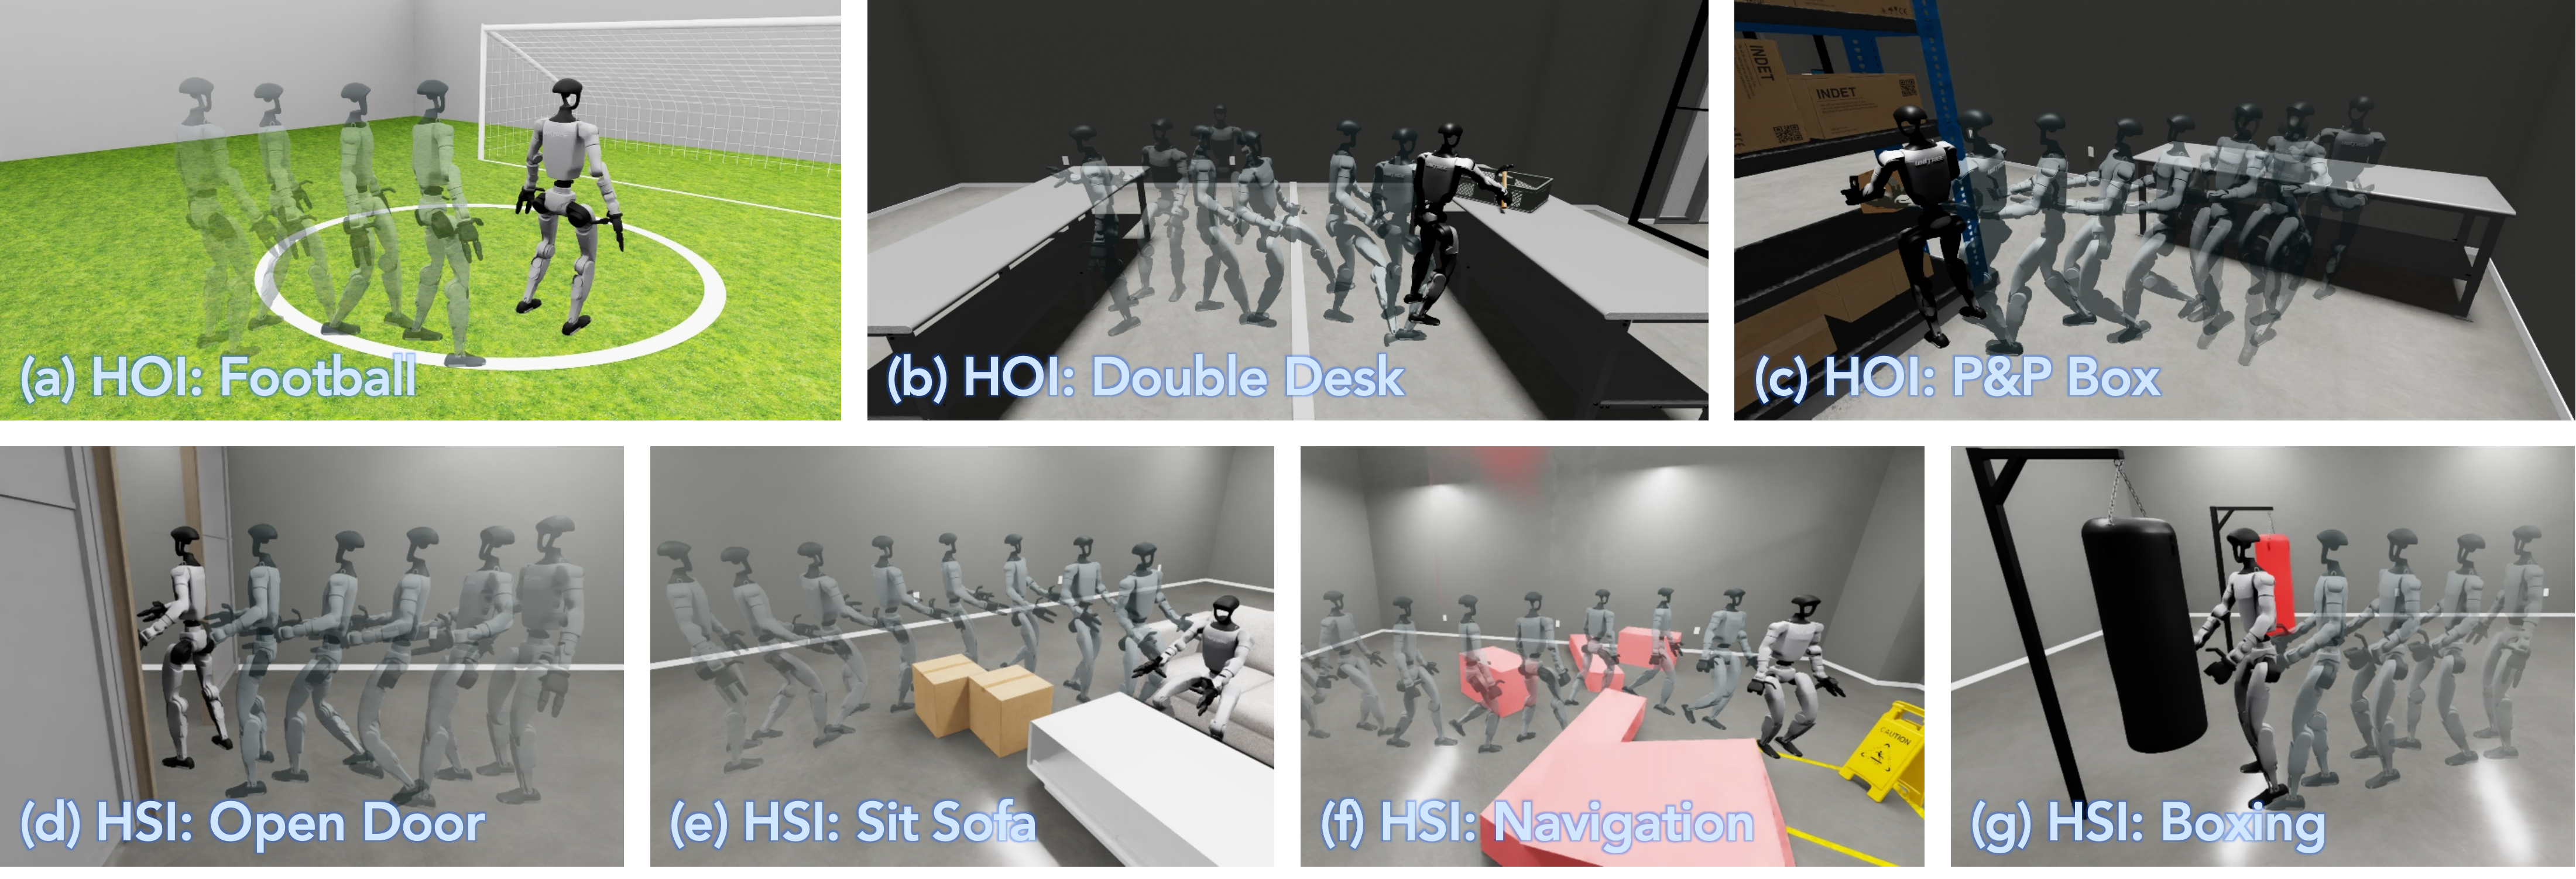
\includegraphics[width=\textwidth]{image/arena.png}
  \caption{\textbf{Visualization of the Seven HumanoidArena Tasks.} The benchmark includes Football, DoubleDesk, P\&Pbox, OpenDoor, SitSofa, Boxing, and VisNavi, covering language-conditioned humanoid behavior across human--object and human--scene interaction with coordinated locomotion, balance, and manipulation.}
  \label{fig:humanoidarena}
\end{figure}

\clearpage
\subsection{SIMPLE Tasks}
\label{sec:vis_simple}

Figure~\ref{fig:simple_tasks} presents the eight evaluated SIMPLE tasks in furnished indoor environments. Handover, Mobile P\&P, and XMoveBendPick combine object handling with positioning relative to the target. CloseDoor, OpenOven, OpenFaucet, and OpenTrashCan involve operating articulated objects, whereas Push Office Chair requires maintaining contact while moving an object through the scene. The panels illustrate variations in target geometry, interaction location, and required body posture. Section~\ref{sec:exp_simple} evaluates these tasks under the L0--L2 protocol to quantify robustness to visual, lighting, and target-pose variation.

\begin{figure}[H]
  \centering
  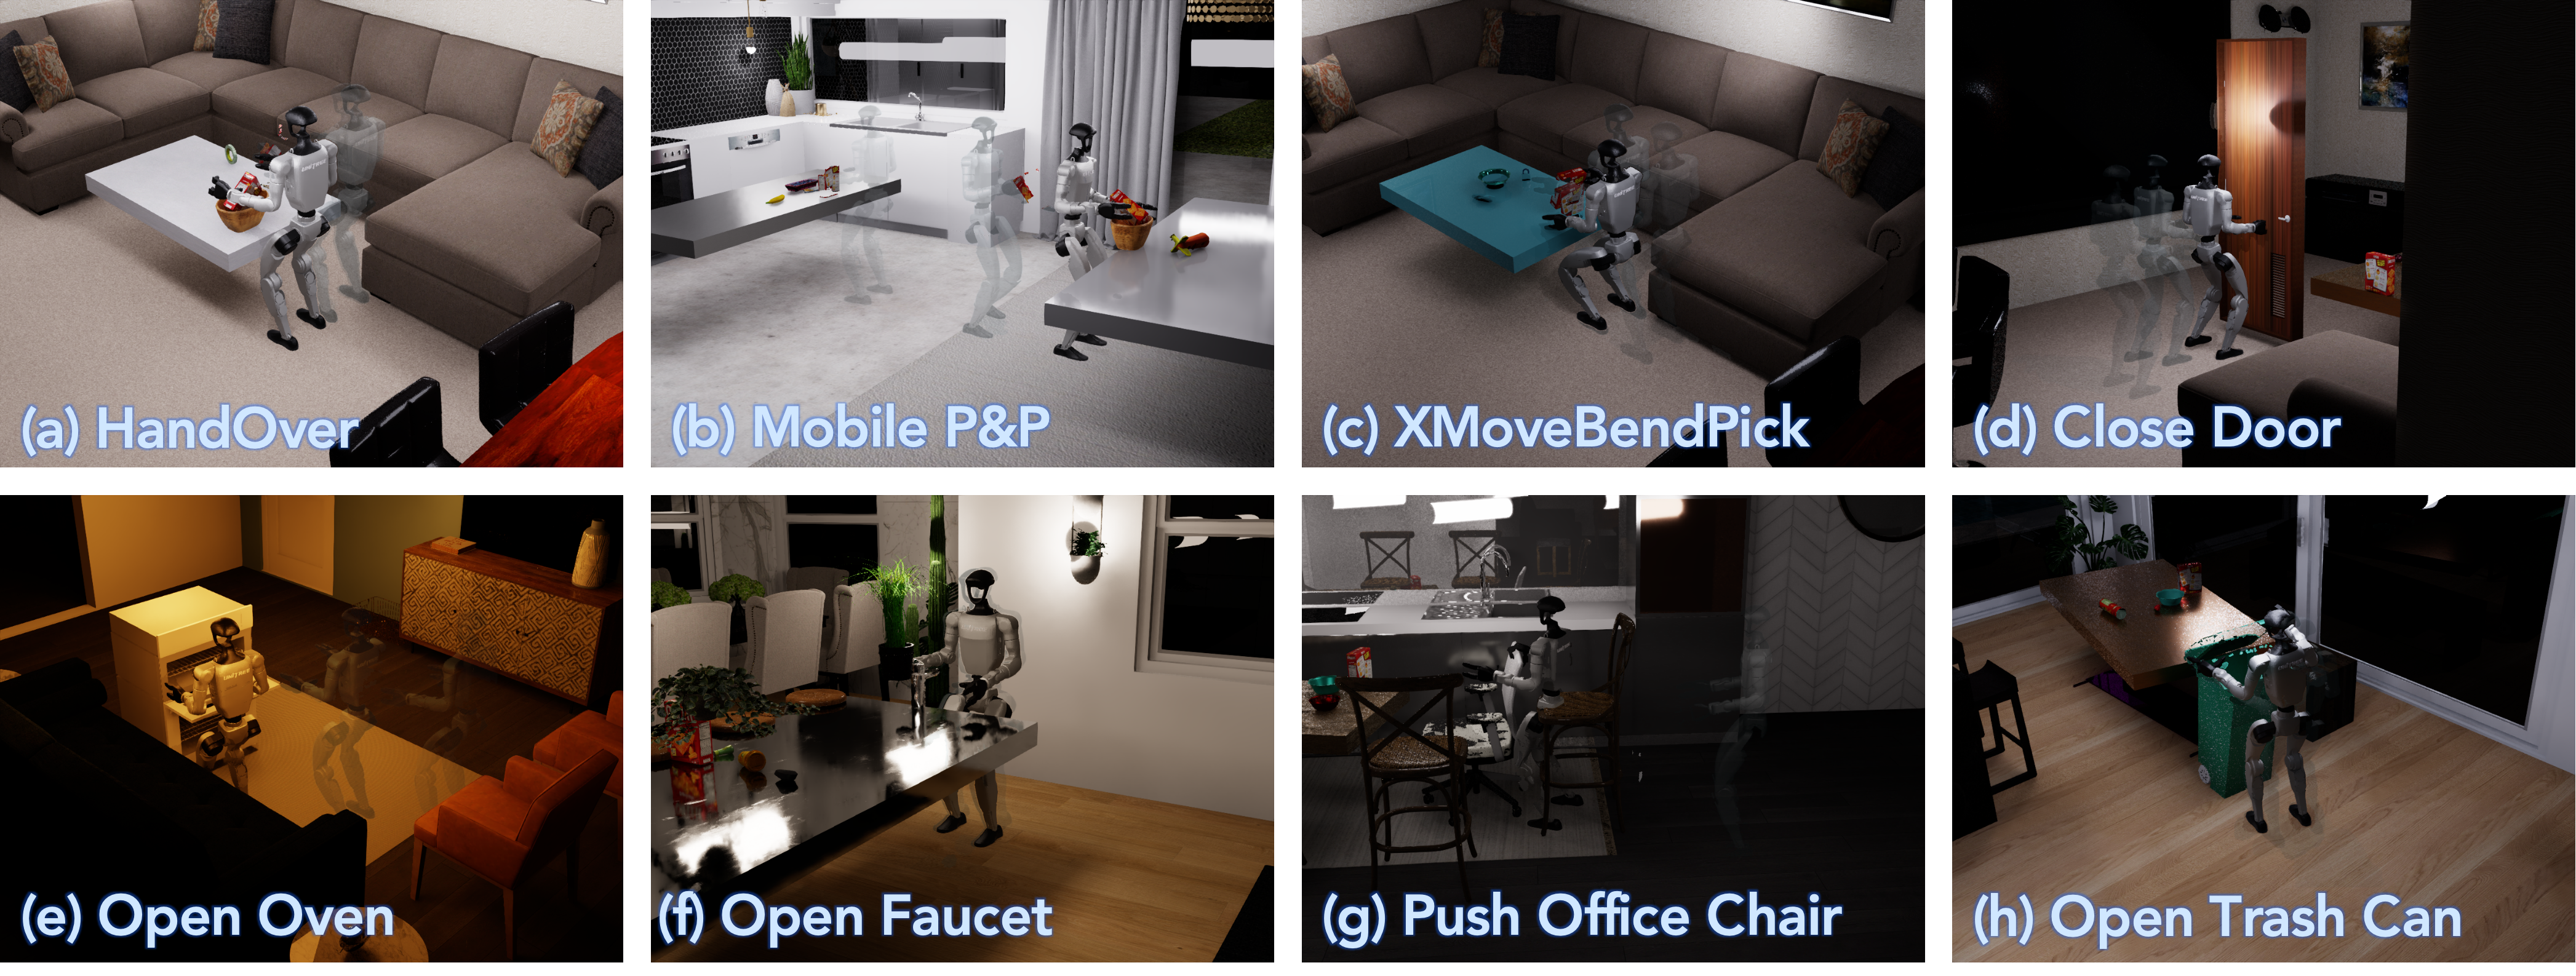
\includegraphics[width=\textwidth]{image/simple.png}
  \caption{\textbf{Evaluated SIMPLE Task Suite.} The selected tasks cover object handover and mobile pick-and-place, locomotion-integrated object pickup, articulated-object interaction, and household-object manipulation. Panels show (a) Handover, (b) Mobile P\&P, (c) XMoveBendPick, (d) CloseDoor, (e) OpenOven, (f) OpenFaucet, (g) Push Office Chair, and (h) OpenTrashCan.}
  \label{fig:simple_tasks}
\end{figure}

\clearpage
\subsection{Real-World Tasks}
\label{sec:vis_real_world}

Figure~\ref{fig:real_world} presents temporally ordered snapshots of the eight real-world tasks, with language instructions specifying the intended interactions. Panels (a--d) show tabletop pick-and-place, cushion sitting, banana placement followed by drawer closure, and apple placement followed by drawer closure. Panels (e--h) show approaching and kicking a ball, sequential interaction with two punching bags, carrying a box to a cabinet, and pushing a cart. Within each panel, the sequence progresses from preparation or approach to interaction and subsequent motion. The accompanying changes in body posture illustrate the coordination of locomotion, reaching, and sustained contact required by these tasks. Quantitative success rates are reported in Section~\ref{sec:exp_real}.

\begin{figure}[H]
  \centering
  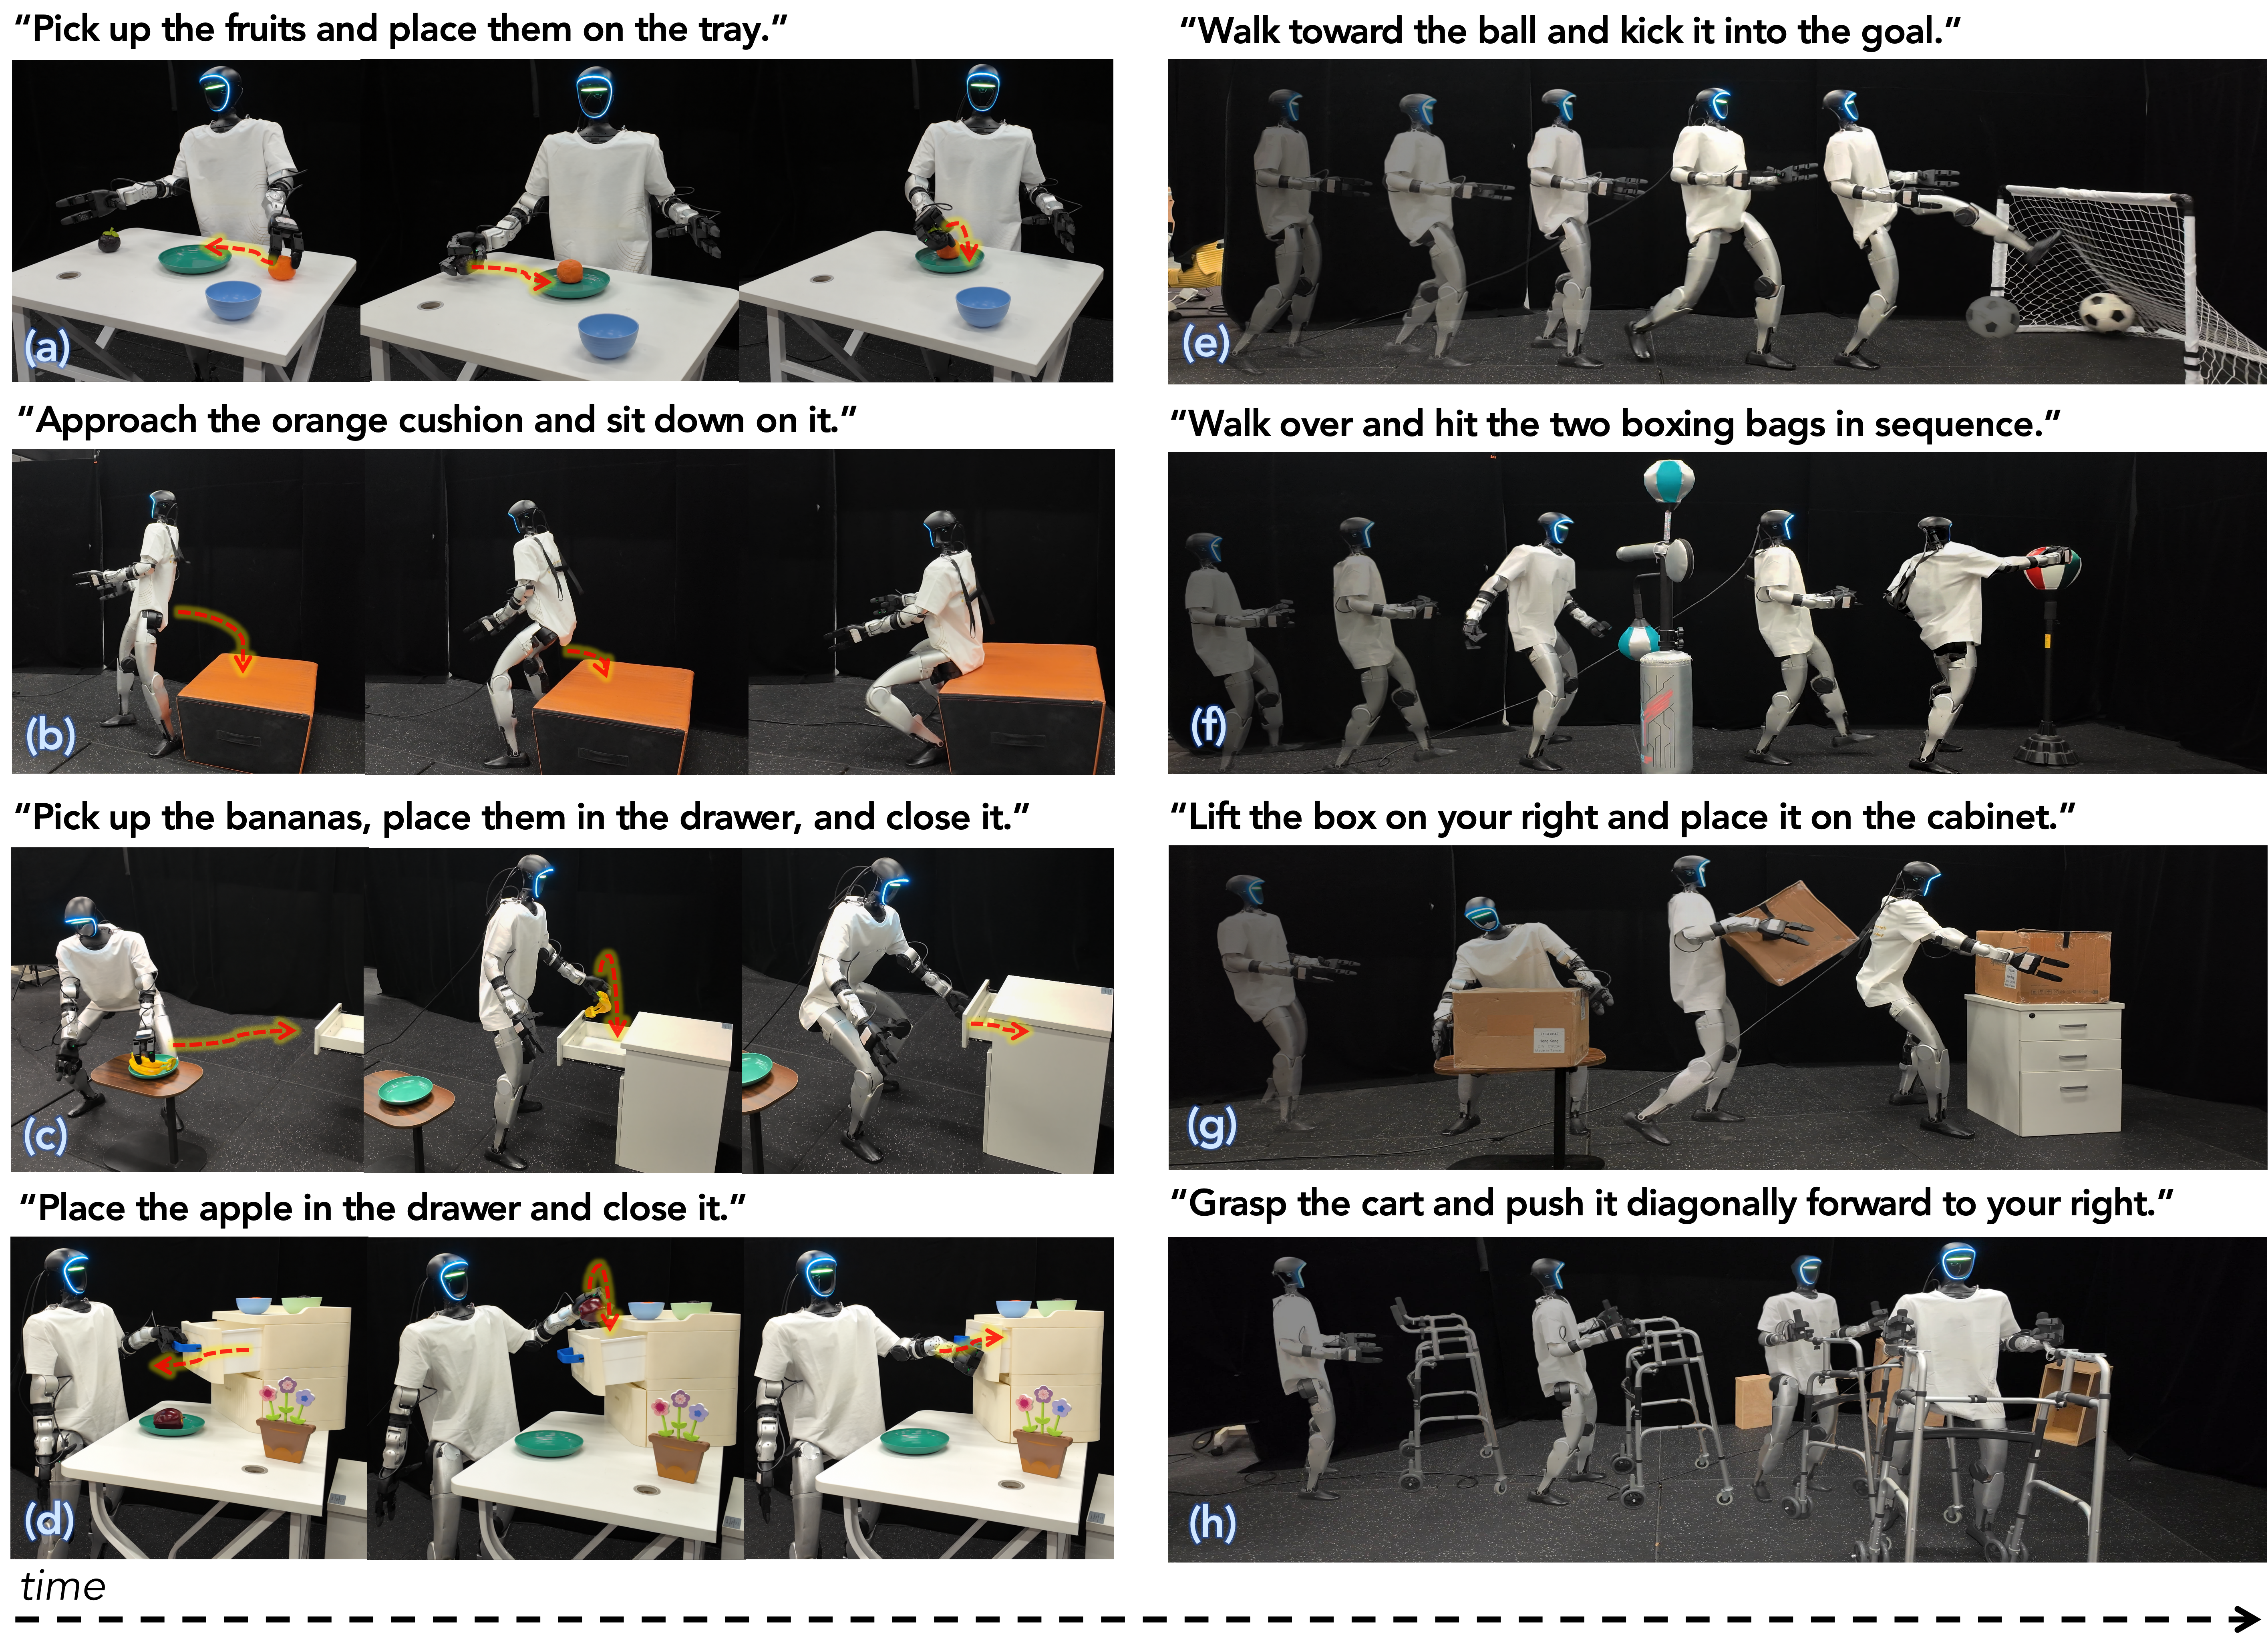
\includegraphics[width=\textwidth]{image/real_world.png}
  \caption{\textbf{Examples of Real-World Humanoid Manipulation.} The image shows representative interaction scenarios involving articulated objects, object transport, and coordinated whole-body motion.}
  \label{fig:real_world}
\end{figure}
